%%%%%%%%%%%%%%%%%%%% author.tex %%%%%%%%%%%%%%%%%%%%%%%%%%%%%%%%%%%
%
% sample root file for your "contribution" to a contributed volume
%
% Use this file as a template for your own input.
%
%%%%%%%%%%%%%%%% Springer %%%%%%%%%%%%%%%%%%%%%%%%%%%%%%%%%%%%%%%%%

\title{Overview of SimCenter Goals and Computational Tools}
% Use \titlerunning{Short Title} for an abbreviated version of
% your contribution title if the original one is too long
\author{
    \textbf{Gregory G. Deierlein}
    \and Frank McKenna
    \and Sanjay Govindjee}
\tocauthor{}
\authorrunning{Deierlein et al.}
% Use \authorrunning{Short Title} for an abbreviated version of
% your contribution title if the original one is too long
%\institute{Name of First Author \at Name, Address of Institute, %\email{name@email.address}
%\and Name of Second Author \at Name, Address of Institute %\email{name@email.address}}
%
% Use the package "url.sty" to avoid
% problems with special characters
% used in your e-mail or web address
%
\maketitle
\label{chapter:intro}

Computational simulation is as an essential component of natural hazards engineering research and practice to assess and mitigate the damaging effects of earthquakes, wind storms and associated tsunami, and storm surge effects on communities. The recently published National Hazards Engineering Research Infrastructure Science Plan \citep{edge2020natural} outlines three grand challenges and five research questions, all of which depend on integration of data and models through computational simulations.  Specifically, simulations are critical to (1) characterize natural hazard phenomena, (2) evaluate their damaging effects on buildings, civil infrastructure and other physical assets, (3) quantify the socio-economic consequences of this damage, and (4) evaluate the effectiveness of alternative strategies to mitigate and recover from the damage.  Each of these components entail simulations at varying scales, from detailed analyses of localized response of individual buildings or infrastructure components to multi-scale analyses of regionally distributed communities and infrastructure systems.  The challenges are multi-disciplinary and require development and management of large datasets to translate data and analysis results between the simulation components. Recognizing the challenge as broad and multi-disciplinary, and encompassing natural hazards across a wide range of scales, the SimCenter’s approach is to leverage existing software platforms by creating computational workflow technologies that can seamlessly integrate a broad array of simulation software with high-performance computing platforms and data repositories. When necessary, the SimCenter also creates new software to implement established theories to achieve its end goals.

\section{SimCenter Application Framework}

The SimCenter’s application framework leverages foundational advancements in performance-based engineering to integrate models and data from the physical sciences, engineering, and social sciences to evaluate and design strategies to create resilient communities \citep{deierlein2020cloud}.  The basic framework of performance-based engineering, illustrated in Figure \ref{fig:intro_PBE_framework}, was originally developed for earthquake engineering design, but the concept is generally applicable to other natural hazards.  Moving from left to right, the process begins with the definition of a constructed facility, based on its design features and location. The next steps are to perform (1) a hazard analysis to characterize the hazard effects (e.g., earthquake ground shaking) that the facility is subjected to, (2) structural analyses to assess the response of the facility to the hazard, (3) damage analyses to quantify damage to facility components associated with the imposed calculated deformations and forces, and (4) consequence analyses to evaluate the resulting risks to life safety, economic losses, and downtime.  Input and output variables from each stage of the assessment are clearly defined as part of an underlying probabilistic formulation to characterize and propagate statistical data through the analyses.

\begin{figure}[htb]
    \centering
    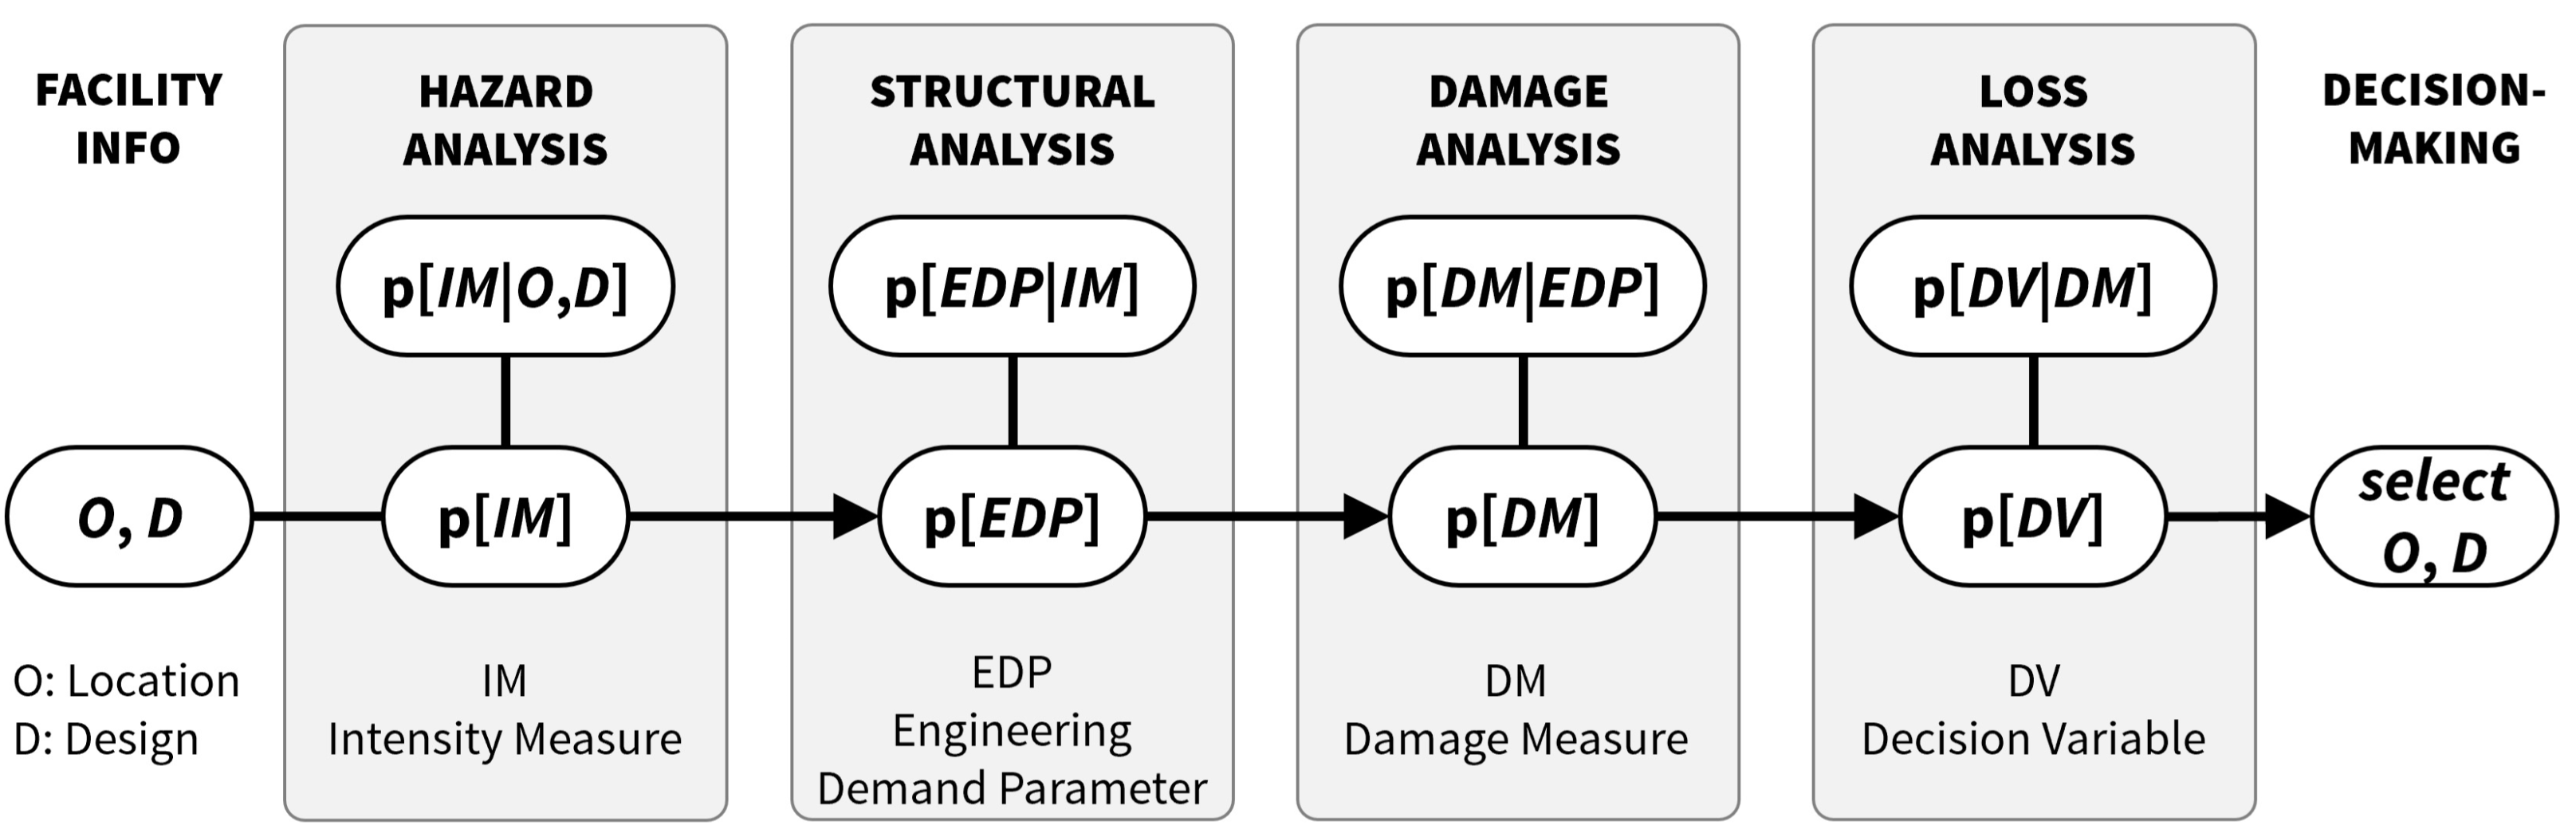
\includegraphics[width=1.0\textwidth, angle = 0]{Figures/PBE_framework.png}
    \caption{Performance-based engineering framework for organizing data transfer between modeling components (after \cite{porter2003overview})}
    \label{fig:intro_PBE_framework}
\end{figure}

As shown in Figure \ref{fig:intro_SimCenter_framework}, computational workflows to implement the performance-based framework can be envisioned as a set of puzzle pieces, each of which encapsulates one or more software components with pre- and post-processing operations to facilitate transfer of data between the components.  The framework allows users to (1) select from different applications for each jigsaw piece, (2) build a computational workflow with the selected components, and (3) then launch and monitor the running workflow. Workflow systems are configured to launch the individual applications and pass the needed input and output data between the applications.  The application framework is designed to be modular and extensible, such that researchers can introduce their preferred application for any step in the process.  Workflows can be configured for end-to-end simulations, from characterization of the natural hazard effects through to damage and impacts on individual facilities or large inventories of facilities, or alternatively for sub-portions of the system.  As illustrated by the top grey bar in Figure \ref{fig:intro_SimCenter_framework}, an important emphasis of the workflows are capabilities to incorporate and propagate inherent variabilities and modeling uncertainties through the computational simulations. Another integrating aspect, illustrated by the lower grey bar in Figure \ref{fig:intro_SimCenter_framework}, is to integrate the computational tools with supporting datasets that support various components of the workflow. 

\begin{figure}[htb]
    \centering
    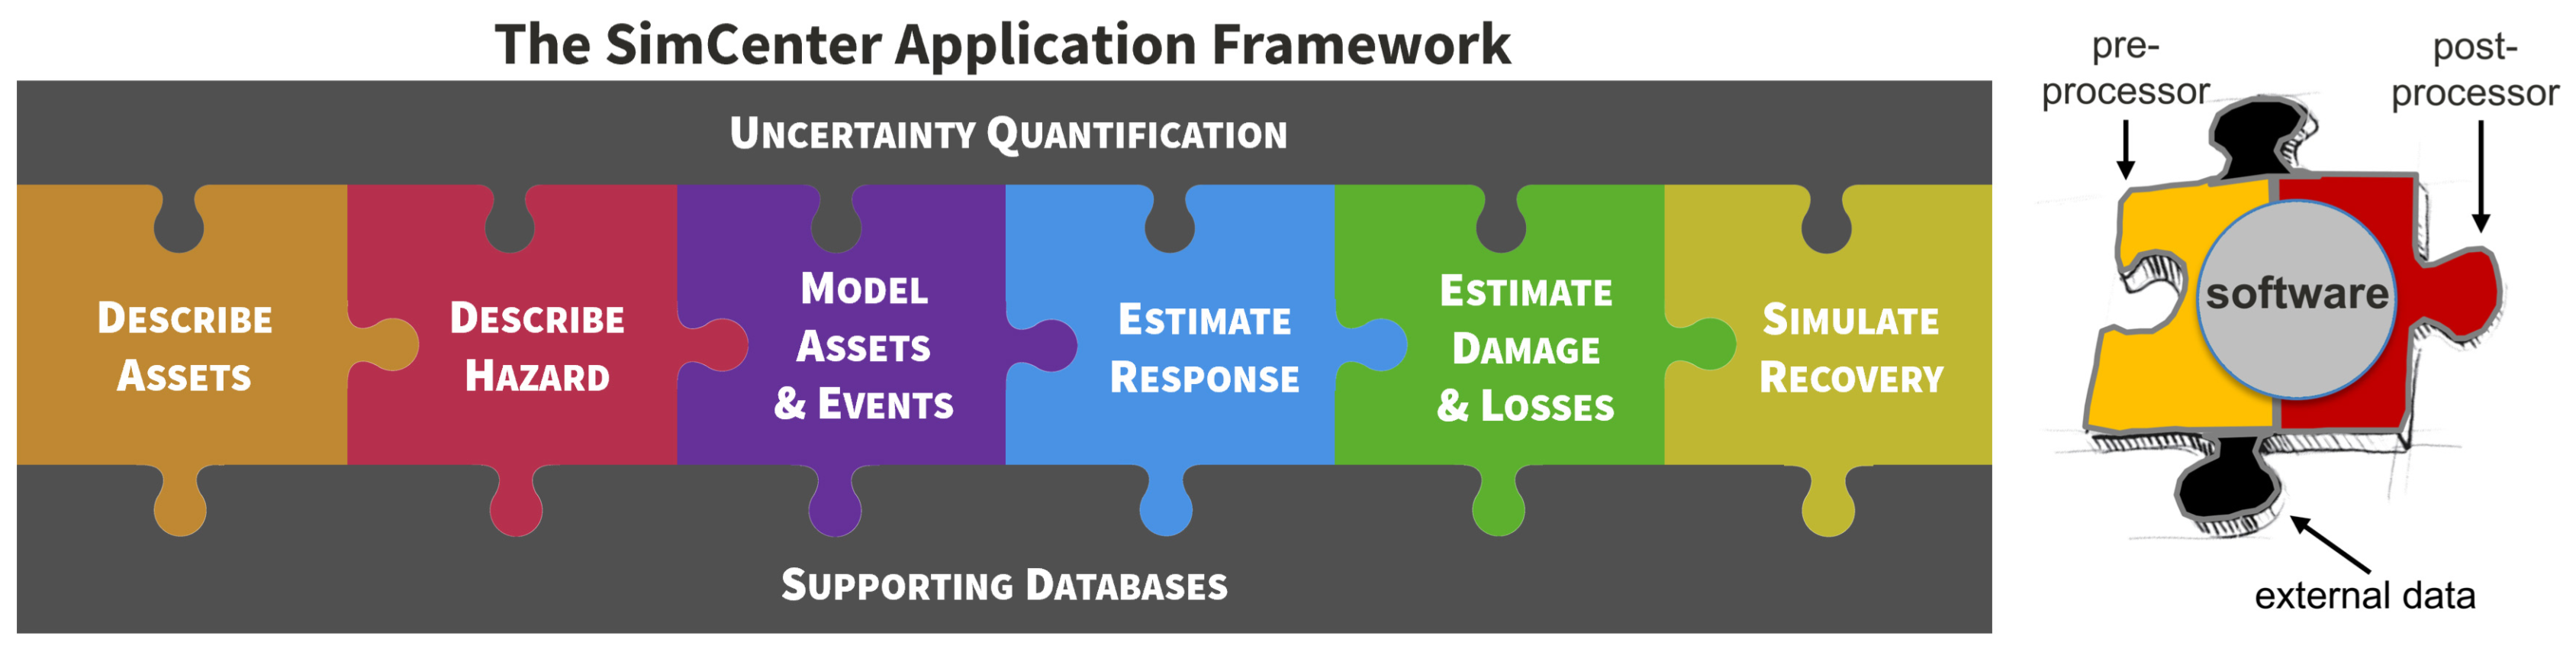
\includegraphics[width=1.0\textwidth, angle = 0]{Figures/SimCenter_framework.png}
    \caption{Modular framework of the SimCenter computational workflow for end-to-end simulations of natural hazard effects on damage and recovery of the built environment and communities}
    \label{fig:intro_SimCenter_framework}
\end{figure}

Figure \ref{fig:intro_SimCenter_tools} illustrates how the conceptual workflow puzzle is abstracted into software components, along with supporting datasets.  The items listed across the bottom of the figure represent key components to the performance-based engineering workflow, and the bins up the right side refer to supporting databases.  The boxes shown higher in the figure are workflow applications that integrate various components of the framework \citep{mckenna2020simcenter}.  Details of these components, databases, and applications are described later.  Figure \ref{fig:intro_SimCenter_integration} illustrates how the SimCenter’s workflow components and applications are integrated into the NHERI cyberinfrastructure system, DesignSafe \citep{rathje2017designsafe}, and other supporting online resources.  As shown in Figure \ref{fig:intro_SimCenter_integration} and described by Rathje et al., DesignSafe provides computing hardware and software infrastructure for online databases and high-performance computing.

\begin{figure}[htb]
    \centering
    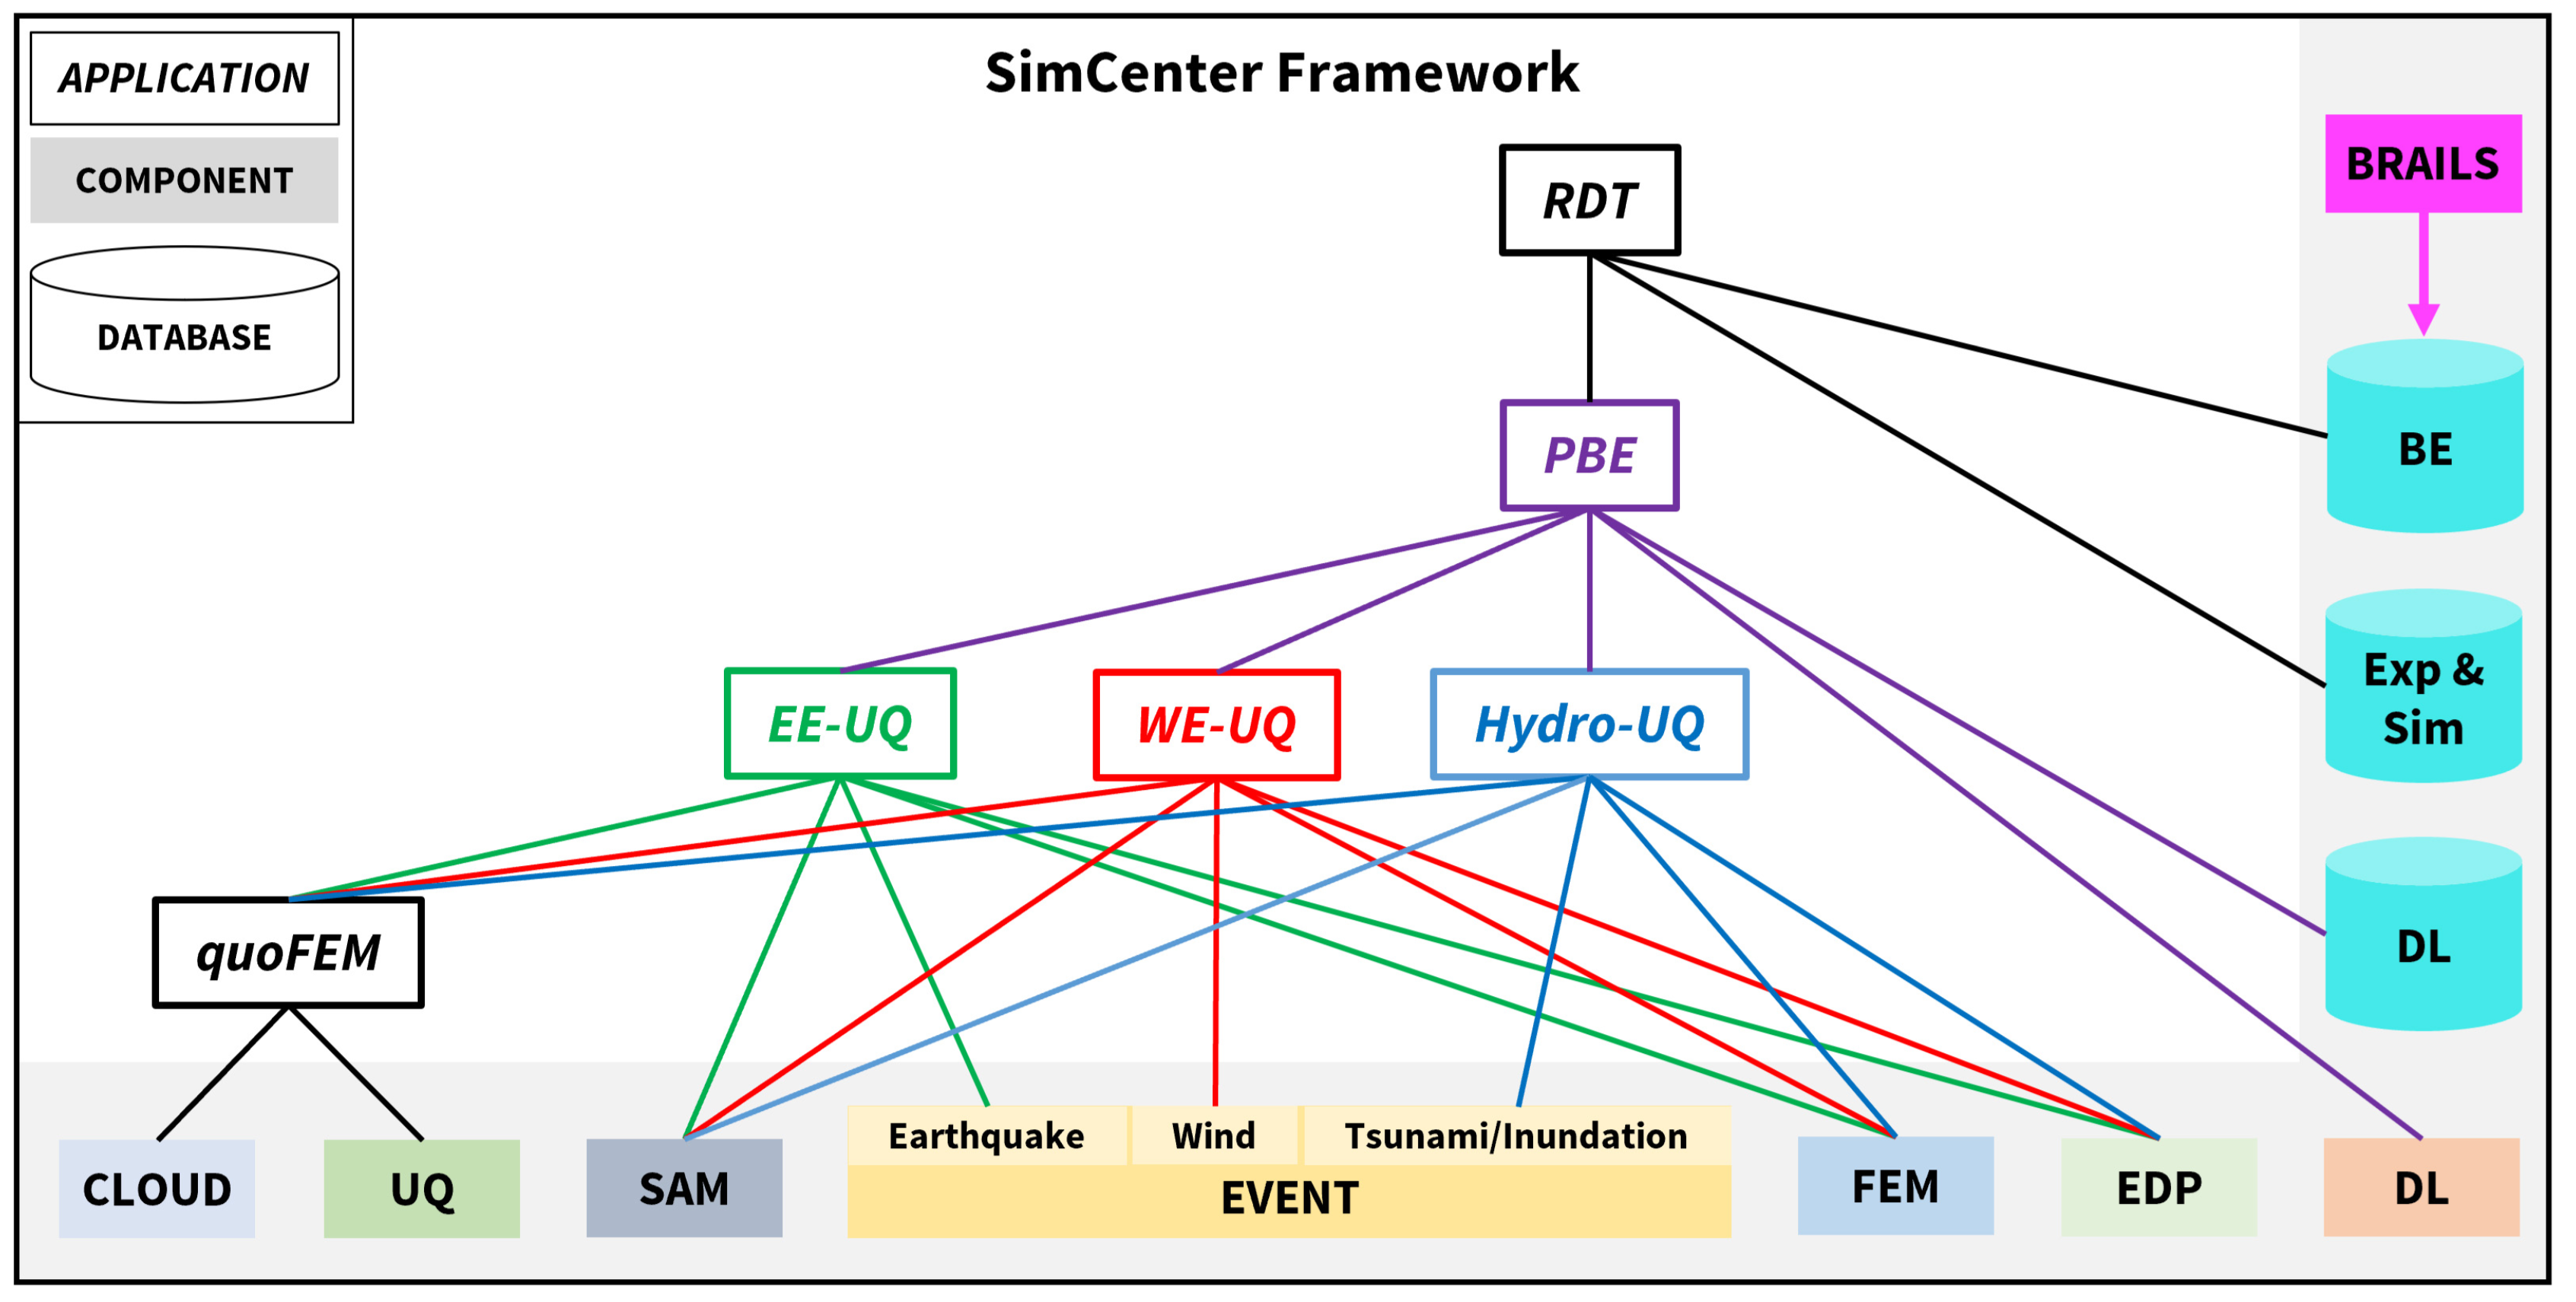
\includegraphics[width=1.0\textwidth, angle = 0]{Figures/SimCenter_tools.png}
    \caption{Schematic diagram of simulation framework components, databases, and application tools}
    \label{fig:intro_SimCenter_tools}
\end{figure}

\begin{figure}[htb]
    \centering
    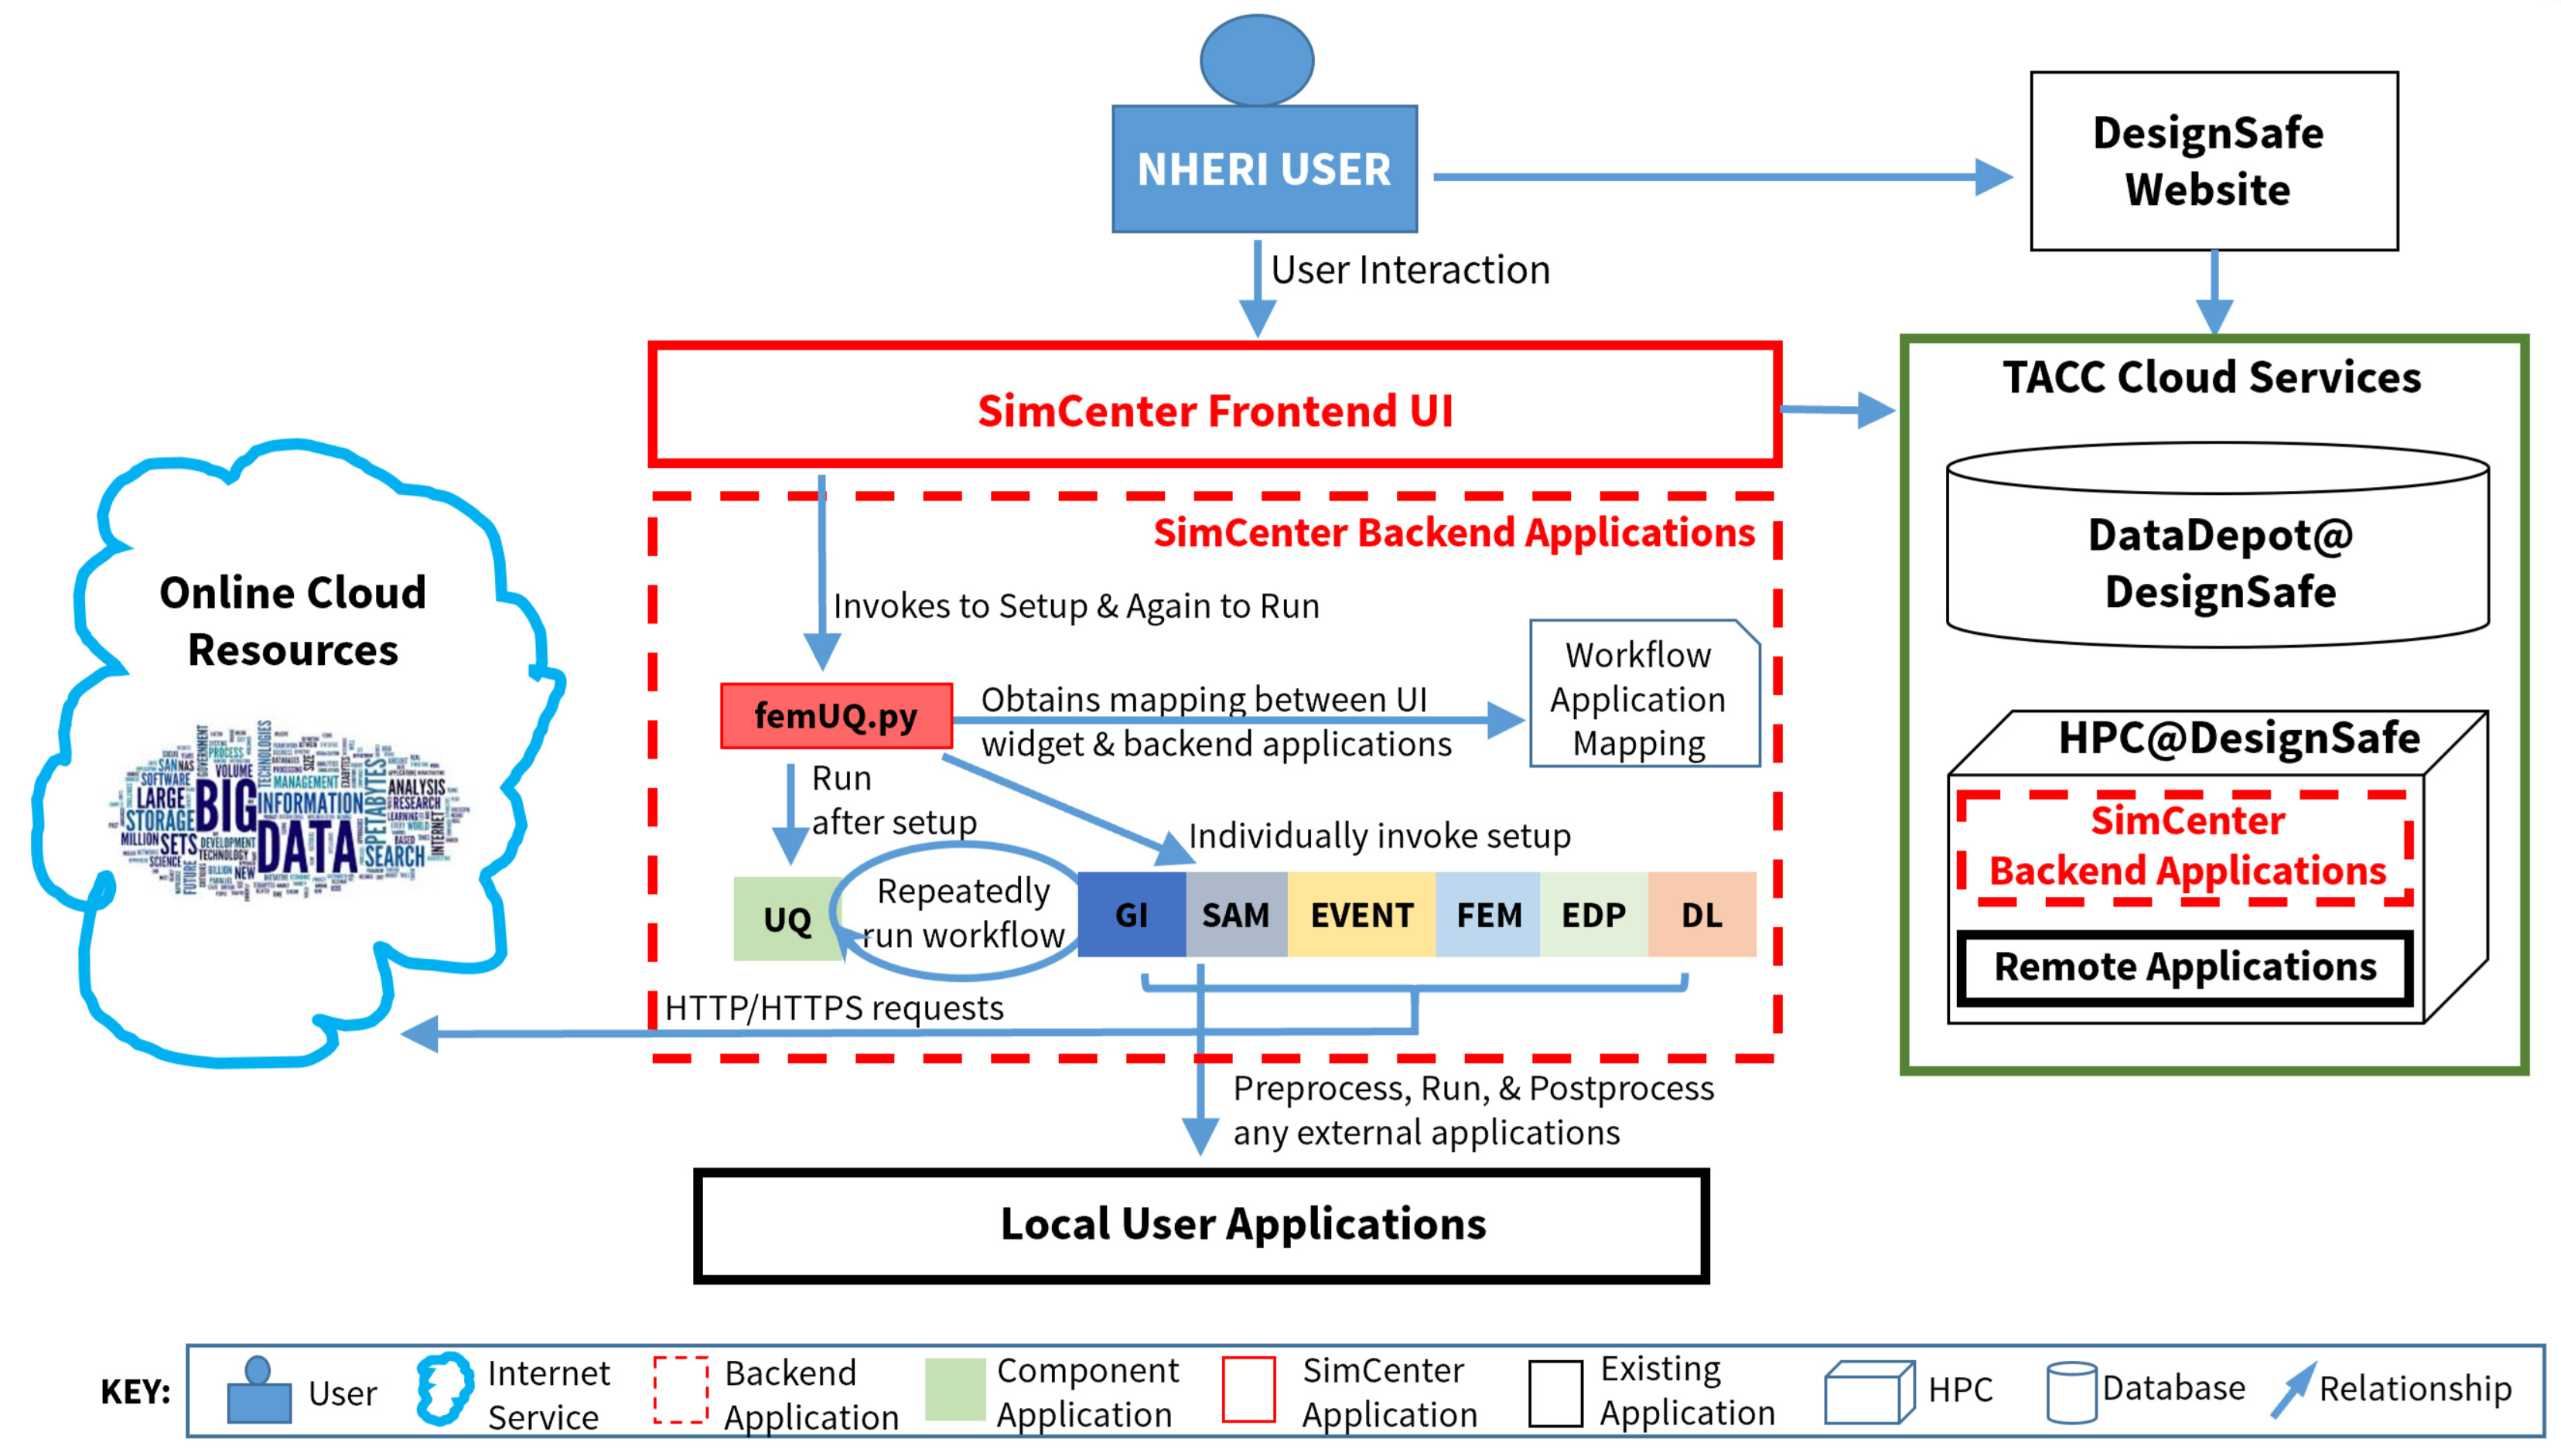
\includegraphics[width=1.0\textwidth, angle = 0]{Figures/SimCenter_integration.png}
    \caption{Integration of the SimCenter workflow tools into the NHERI Computational Environment}
    \label{fig:intro_SimCenter_integration}
\end{figure}

\section{SimCenter Framework Components}

The following is a description of the modeling components and databases of the SimCenter framework shown in Figure \ref{fig:intro_SimCenter_tools}: 

\paragraph{BE – Built Environment Inventory} The BE consists of meta-data and data files that define the inventory of physical assets for a regional simulation, including buildings, transportation components and systems, utility infrastructure components and systems, etc.  By providing a framework to organize and store databases on Design Safe, the SimCenter aims to promote best practices for collection and sharing inventory data. To help facilitate development of inventories, the SimCenter has developed artificial intelligence (AI) tools for building inventory data collection (BRAILS – Building Recognition using AI at Large Scale \citeprgm{wang2019brails}) and for data enhancement (SURF – Spatial Uncertainty Research Framework \citeprgm{wang2019surf}), along with web data query/collection techniques. 

\paragraph{EVENT – Hazard Event} The EVENT consists of meta-data and data files that define the hazard data (e.g., earthquake ground motions, wind fields, storm surge inundation, tsunami inundation).  For earthquake hazard studies, the SimCenter workflow tools include software applications for (i) generating earthquake target spectra from the USGS OpenSHA web service, (ii) selecting and scaling recorded ground motions from the PEER NGA database, (iii) generating simulated stochastic ground motions, and (iv) ingesting simulated ground motions from databases of simulated and recorded ground motions.  For wind and storm surge studies, the workflow can support (i) generating wind field time histories stochastically or using OpenFOAM \citeprgm{openFOAM}, (ii) incorporating experimental wind tunnel datasets utilizing online resources such as Vortex Winds \citep{kareem2017cyber} and the TPU Aerodynamic Database \citep{tpu2020tpu}, or a user’s own local dataset, and (iii) interfaces for querying and ingesting wind speeds and storm surge inundation heights from external applications.

\paragraph{SAM – Structural Analysis Model} The SAM is the workflow component that includes rule-based, AI and other types of applications to translate descriptive information from the built environment inventory into information to create finite element or other types of models to simulate the structural response to the hazard effects. 

\paragraph{FEM – Finite Element Modeling} The FEM module consists primarily of wrappers for input/output to  existing finite element software to simulate the response of structures and geotechnical materials to earthquake ground shaking, wind, storm surge wave loading, and tsunami wave loading.  Such analyses could also encompass computational fluid dynamics and structure-fluid interaction.  OpenSees \citeprgm{OpenSees} and OpenFOAM \citeprgm{OpenFOAM} are the main open source applications that are called by the current FEM wrappers.

\paragraph{EDP – Engineering Demand Parameters} The EDP represents the workflow component that defines and manages the output of hazard-induced deformation or other demands from a finite element or other type of analysis model for input into the damage and loss assessment.

\paragraph{DL – Damage and Losses}  DL is the workflow component where damage and losses are calculated for the assets in the built environment inventory. Since these calculations are essential to all performance assessments and not readily available in existing software, the SimCenter developed an application framework called PELICUN, Probabilistic Estimation of Losses, Injuries and Community Resilience Under Natural Disasters, (\cite{zsarnoczay2020pelicun}, \citeprgm{PELICUN}) to generalize the FEMA P-58 methodology to evaluate damage and losses in buildings and other facilities under earthquakes, hurricanes and other hazards. 

\paragraph{UQ – Uncertainty Quantification} The UQ component provides an interface to software and routines for methods of uncertainty quantification, which can be interfaced with other components.  One of the registered applications supported by UQ is DAKOTA \citep{adams2009dakota}, which offers a range of methods for uncertainty quantification. Additional UQ algorithms are provided by custom SimCenter software.

\paragraph{Cloud} Cloud is the workflow component that manages communication with remote computing and data service providers and sending/receiving data over the web.

\paragraph{DL Data} DL Data is the component consisting of databases of fragility curves for damage and loss calculations for various types of facilities (buildings, bridges, infrastructure) subjected to demands from various hazards (earthquake, wind, surge).

\paragraph{Exp/Sim Data} Exp/Sim Data is the component consisting of databases of experimental and/or computational research data that is utilized for machine learning SAM applications and validation of FEM simulation tools.

\section{SimCenter Desktop Applications and Backend Tools}

Shown in Figure \ref{fig:intro_SimCenter_tools} are the key desktop applications (\emph{quoFEM}, \emph{EE-UQ}, \emph{WE-UQ}, \emph{HydroUQ}, \emph{PBE}, and \emph{RDT}) with linkages to the underlying components used by each application. The workflow components are implemented into backend software modules and can be combined in multiple ways.  The table in Figure \ref{fig:intro_tool_overview} lists the SimCenter’s current desktop applications and backend software modules, along with a set of educational applications.  The columns of the table indicate how the various applications and software modules are related to the various hazards and stages of the performance-based engineering framework. Included below are brief descriptions of the desktop applications.  For further details on these applications, along with details on the backend modules and educational applications, the reader is referred to the SimCenter website, \url{https://simcenter.designsafe-ci.org/}. 

\paragraph{quoFEM}  The Quantified Uncertainty with Optimization for the Finite Element Method (quoFEM) application facilitates uncertainty quantification, model calibration, optimization and sensitivity analyses of structural and geotechnical materials, components, and systems by combining existing finite element applications with uncertainty quantification (UQ) applications. The current (V2.2.0) release links two finite-element codes (OpenSees, OpenSeesPy, or FEAPpv) with uncertainty quantification functions in DAKOTA. A graphical user interface is provided with basic functionality to define random variables in the finite-element models and invoke select UQ methods from DAKOTA. Running through the HPC capabilities of DesignSafe, or on a user’s desktop computer, the system makes available unprecedented capabilities for natural hazards researchers to perform UQ simulations. Future planned releases include extensions to include links to other analysis that are running on DesignSafe (e.g., LSDyna) and other uncertainty quantification toolboxes (e.g., UQ-Pyt, UQpy), including options for advanced surrogating methods. The application treats both forward and inverse problems.

\paragraph{EE-UQ} The Earthquake Engineering with Uncertainty Quantification (EE-UQ) application has features to determine the response of a structural and soil-structure systems to earthquake excitations. The current (V2.2.0) release focuses on quantifying the uncertainties in the structural response, given that the properties of buildings (or other structures) and the earthquake events are not known precisely, and that many simplifying assumptions are present in the numerical models (epistemic uncertainties).  By embedding features of the \emph{quoFEM} tool, \emph{EE-UQ} enables the user to specify statistical distributions of the model input parameters, then Monte Carlo and other sampling methods are used to characterize the output. The tool has features to select and input ground motions to match specified earthquake hazard targets. Work is underway to extend \emph{EE-UQ} to include soil-structure interaction models where rock ground motions are propagated through nonlinear soil models into the structural system.

\begin{figure}[htb]
    \centering
    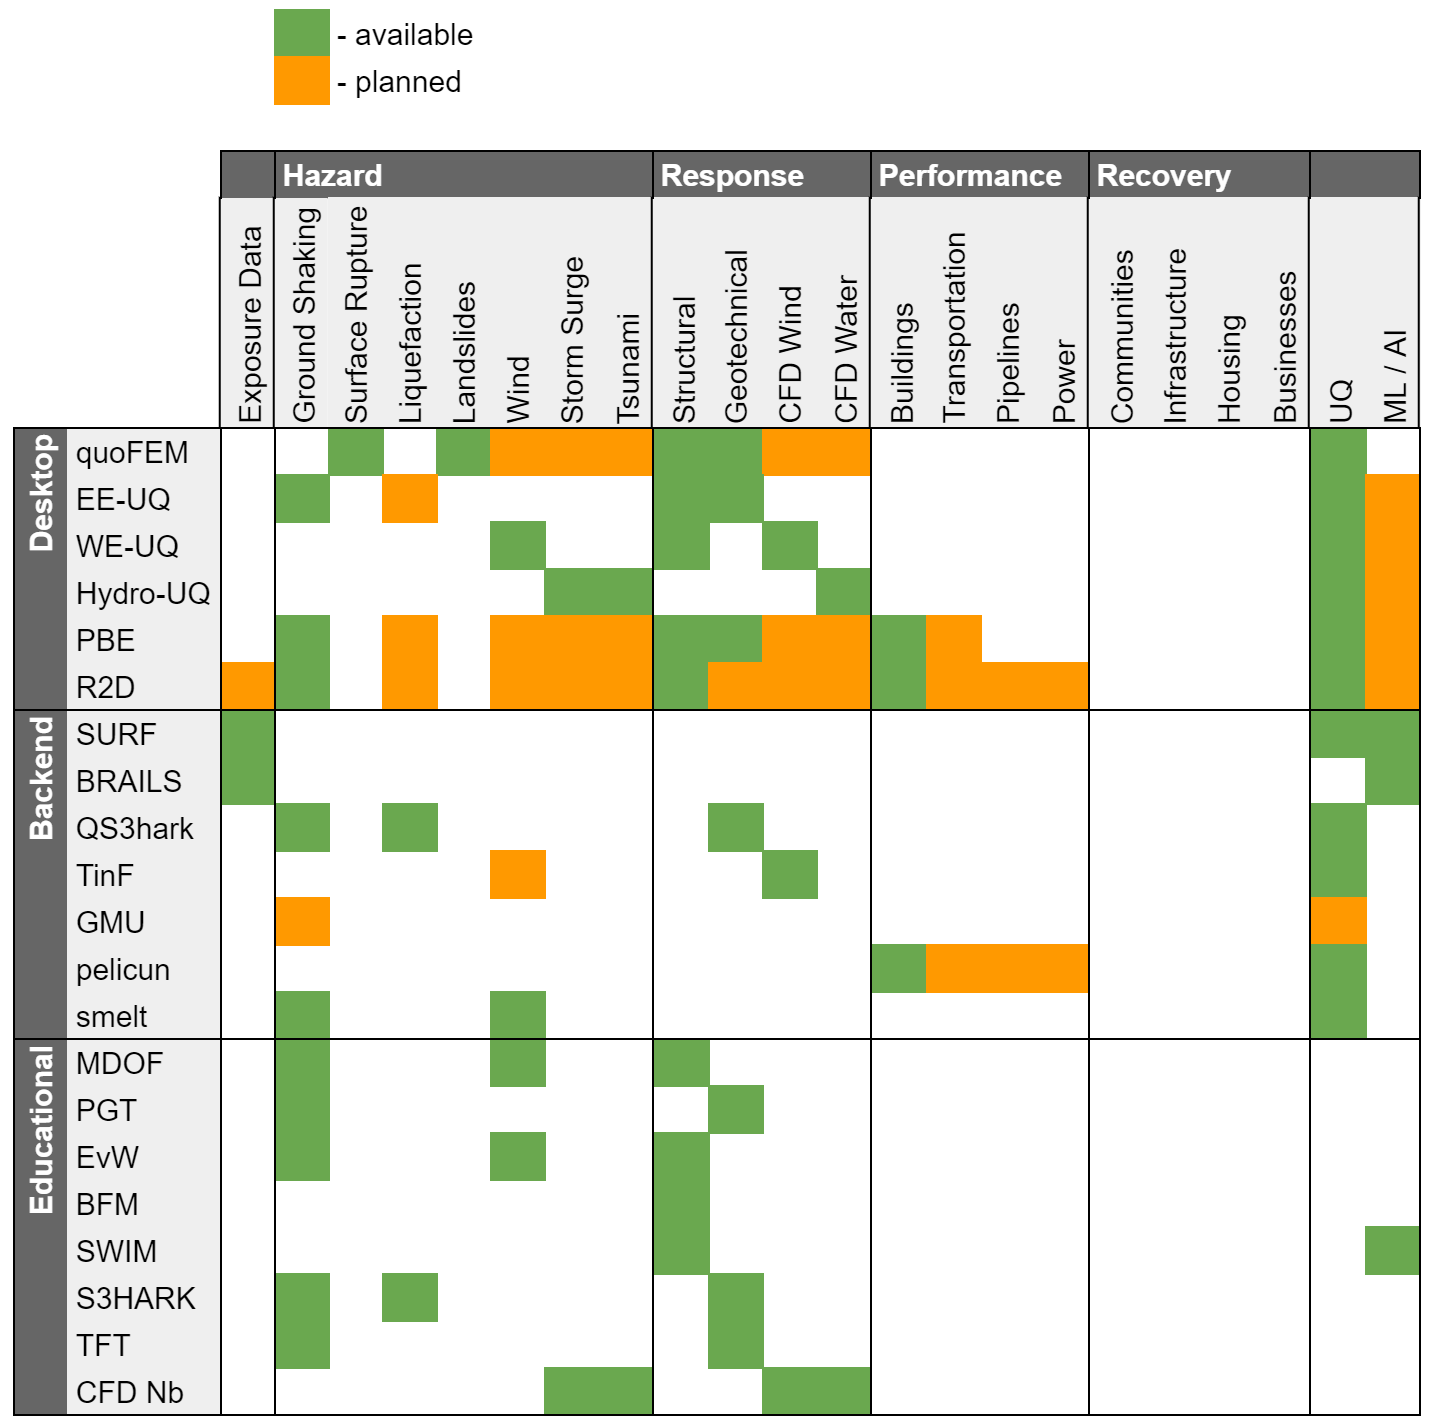
\includegraphics[width=0.75\textwidth, angle = 0]{Figures/tool_overview.png}
    \caption{Overview of SimCenter computational simulation tools}
    \label{fig:intro_tool_overview}
\end{figure}

\paragraph{WE-UQ} This is a wind engineering with uncertain quantification (WE-UQ) application to assess the response of buildings to wind loading, taking into account that the properties of the building and the wind loads are not known exactly, and given that the simulation software and the user make simplifying assumptions in the numerical modeling of the structure. It is similar in composition to \emph{EE-UQ}, but with a wind \emph{EVENT} component.  The current (V2.0.0) version allows users to select from a variety of options for specifying wind forces on structures from stochastic loading models and online wind engineering databases through to performing Computational Fluid Dynamics (CFD) analyses utilizing OpenFOAM. The tool is intended to make detailed CFD modeling more accessible to NEHRI researchers in conjunction with wind tunnel testing (e.g., to validate computational models and extrapolate beyond the scale and parameter space that can be tested in the NHERI wind facilities), to allow researchers to consider more realistic conditions from field studies, and assist in the creation of surrogate models for regional simulations. 

\paragraph{Hydro-UQ} This is a water engineering with uncertainty quantification (Hydro-UQ) application to assess the response of structures to fluid flows from storm surge, tsunamis, or other hazards. The current version (V0.9.0-alpha) allows 2-D shallow water solutions obtained from far-from-coast calculations as input to a 3-D CFD solver. This facilitates a multiscale coupling by resolving areas of interest by coupling shallow-water solvers with CFD solvers through an interchangeable workflow. As a part of the inputs, the tool allows the researchers to consider: (a) bathymetry / topography of the ocean floor (b) initiation conditions due to tsunami / storm surge events. 

\paragraph{PBE} The performance-based engineering (PBE) application is an extensible workflow application to evaluate the performance of buildings or other assets to natural hazards. The current (V2.0.0) release provides researchers a tool to assess the performance of a building subjected to earthquake ground motions. The application focuses on quantifying nonlinear building response and damage through decision variables. \emph{PBE} builds upon the \emph{EE-UQ} tool using the estimates of structural response to assess the damage to building components and the consequences of such damage. The user characterizes the simulation model, and the damage and loss models of the structure, and the seismic hazard model in the \emph{PBE} tool. The tool incorporates an underlying workflow application \emph{PELICUN}, which is modeled after the FEMA P58 framework for earthquake loss assessment but with a broader vision to address alternate hazards (wind, water inundation, etc.) and facilities beyond buildings. 

\paragraph{RDT} The Resilience Decision Tool (RDT) application is an extensible workflow application to quantify the effects of hazards on regional communities. Upon its release (in early 2021) it will provide options for selecting regions, hazards, and viewing the results at a regional scale. The tool will utilize and incorporate the same workflow components used for \emph{WE-UQ}, \emph{EE-UQ}, and \emph{PBE} tools, extended to consider multiple facilities and regionally distributed hazards. As part of the development of the tool, two command line workflow applications are being developed and made available: (1) the Regional Earthquake Workflow and (2) the Regional Hurricane Workflow.  The application has been utilized in two application testbed studies, one focused on earthquake effects on buildings in the San Francisco Bay Area, and the second focused on wind and storm surge effects on buildings in Atlantic City, NJ.

\section{Concluding Remarks}

In addition to developing and releasing the computational workflow tools and training modules, the SimCenter is engaging with researchers to extend the simulation capabilities through collaboration with NHERI researchers. Collaboration opportunities include: (1) development and implementation of new computational simulation models, metadata standards, and software, (2) application studies to apply and enhance the simulation tools across a spectrum of scales – from individual components through to regional studies of the impact of natural hazards on the built-environment, (3) development of educational resources, including curricula materials that utilize advanced simulation tools, along with webinars, papers and other means of documentation. 

This report is an important component of the SimCenter’s workplan to identify and incorporate state-of-the-art simulation methods and software into the computational workflow applications. It also identifies areas where further research and development is needed.  Thus, this report thus serves not only as a state-of-the-art report for the NHERI community but also as a guiding document for the SimCenter.  As seen in Figure \ref{fig:intro_tool_overview}, for example, there is currently a major gap in computational models for simulating disaster recovery, which represents a major challenge to the NHERI community.  Beyond incorporating existing and emerging simulation tools into the computational workflows, an important component of the SimCenter’s work is to overcome computational challenges associated with scaling up the simulations to allow higher fidelity and higher resolution models.  These computational aspects of the software development involve collaboration and coordination with NHERI cyberinfrastructure available through DesignSafe and other organizations. 